\newpage
\section{Các thành phần trong code}
\subsection{Tổng quan về code}

\paragraph{Cấu trúc}
\paragraph{}{Các thành phần trong game được tổ chức như hình bên dưới:}
\begin{figure}[H]
    \centering
    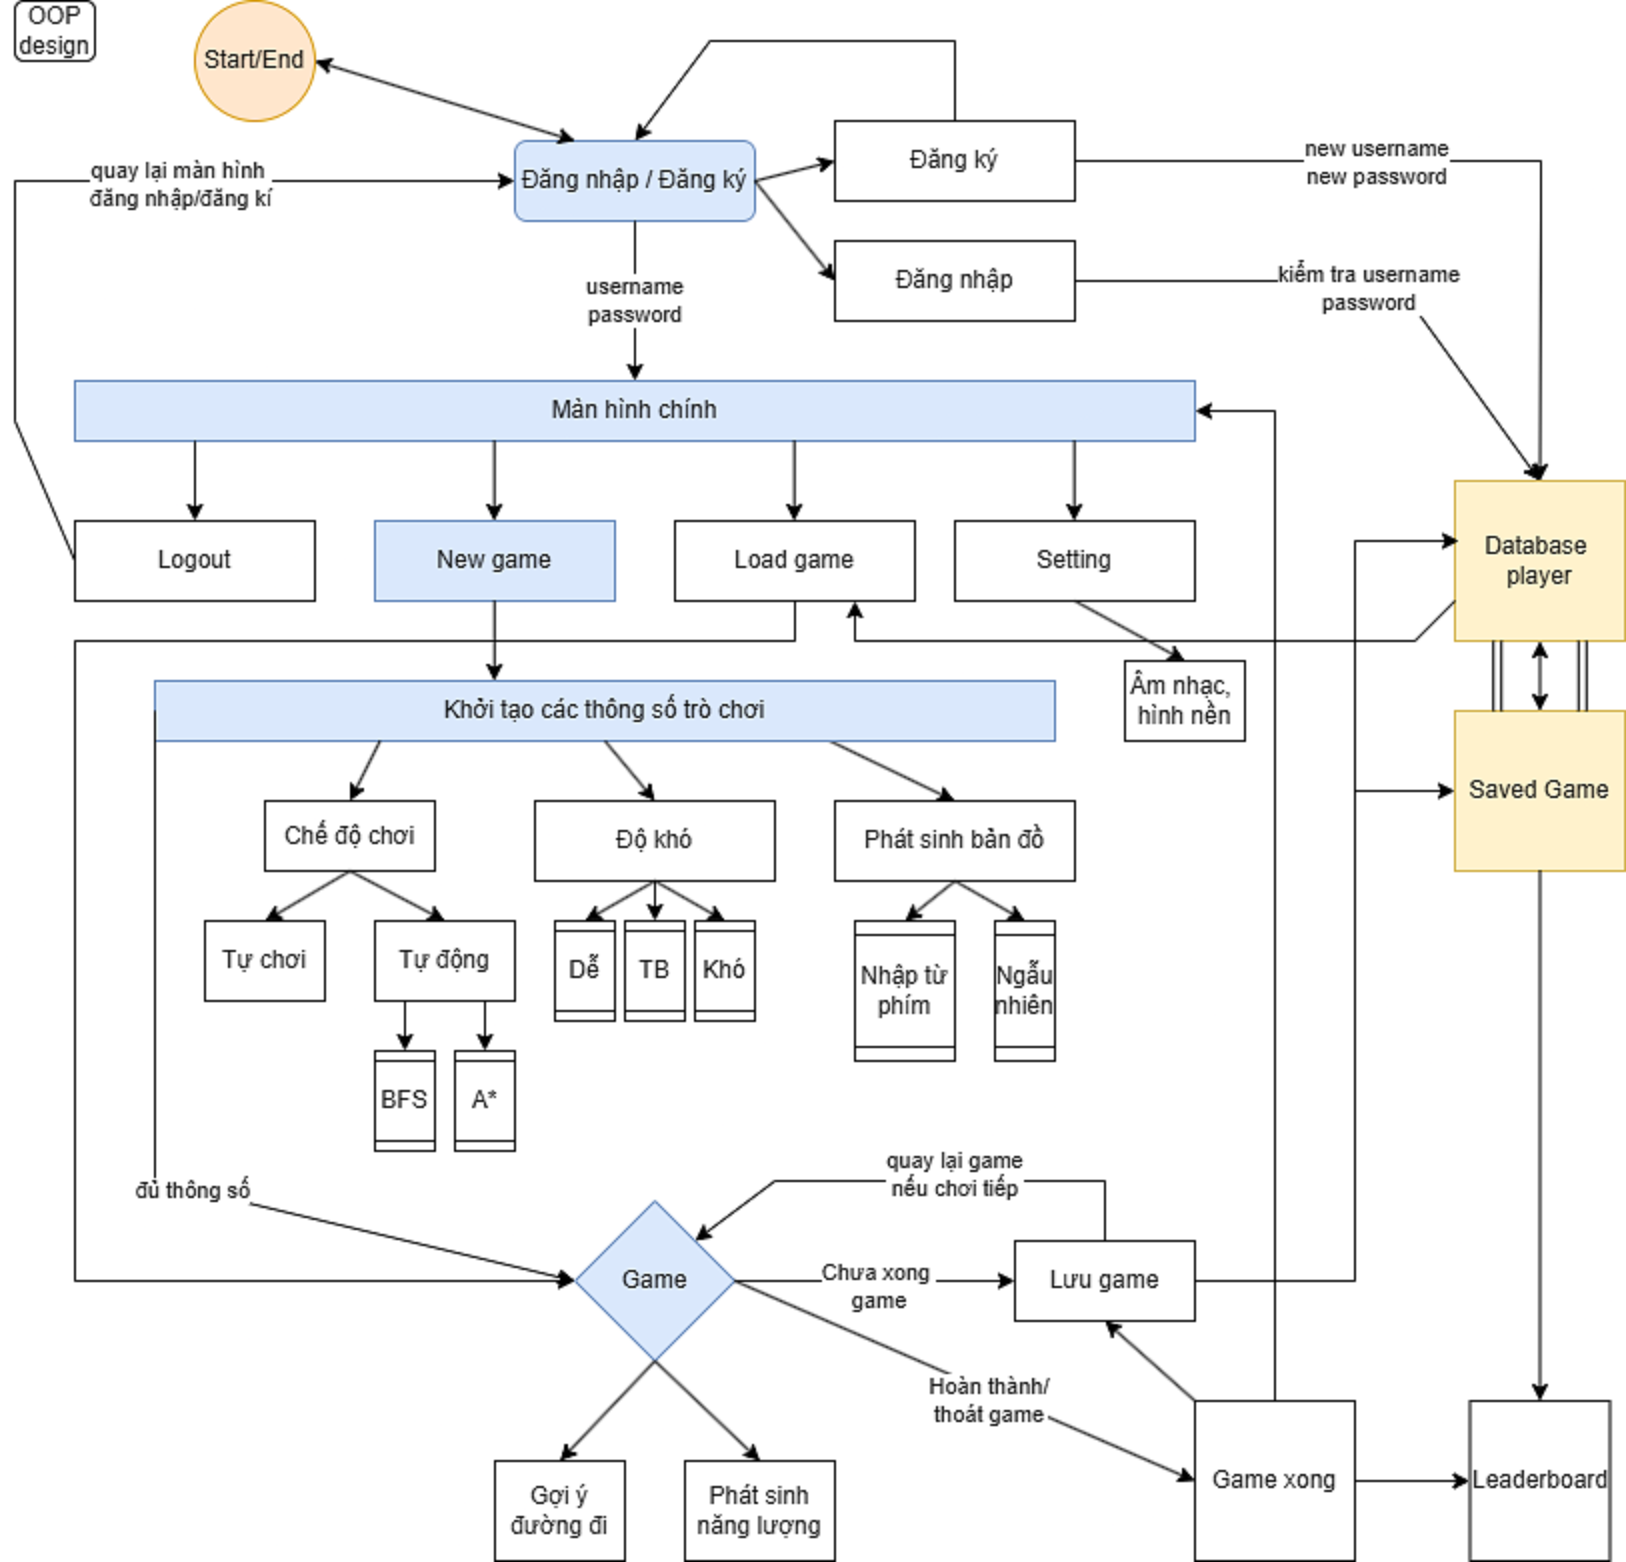
\includegraphics[width=1\linewidth]{img/pj_code.png}
    \caption{Sơ đồ tổ chức code}
    \label{fig:pj_code}
\end{figure}
\newpage

\paragraph{Phương pháp lập trình}
\paragraph{}{Code trong đồ án được tổ chức theo phương pháp lập trình hướng đối tượng. Điều này giúp code rõ ràng, rành mạch, không bị chồng chéo các biến và chức năng với nhau.}

\paragraph{Tổ chức code}
\paragraph{}{Code được tổ chức thành các file với đuôi $.py$. Mỗi file chứa các class, chịu trách nhiệm cho các chức năng riêng, trong đó:}
\begin{itemize}
    \item \textbf{main.py} : Gọi các tệp tin và class khác, khởi tạo trò chơi.

    \item \textbf{database.py} : Lưu trữ thông tin người dùng, các ván chơi và xử lí xuất nhập thông tin, gồm 1 class: \texttt{UserDatabase}

    \item \textbf{login\_startgame.py} : Xử lí giao diện đăng kí, đăng nhập, menu, gồm 2 class: \texttt{LoginMenu}, \texttt{MenuGame}

    \item \textbf{maze\_generator.py} : Khởi tạo các thuộc tính cho mê cung, gồm 2 class: \texttt{Cell}, \texttt{Maze}

    \item \textbf{maze\_solver.py} : Tìm đường đi cho mê cung, gồm 2 class: \texttt{priority\_queue}, \texttt{mazeSolver}

    \item \textbf{utils.py} : Xử lí thông tin của 1 thư mục, gồm 1 hàm \texttt{import\_folder}

    \item \textbf{tile.py} : Hiển thị hình ảnh lên một ô / màn hình (đường đi, gợi ý, đường thuật toán tìm kiếm...), gồm 3 class: \texttt{Goal}, \texttt{Hint}, \texttt{Auto}.

    \item \textbf{Display.py} : Tạo các nút bấm, đồng hồ, hộp văn bản, gồm 5 class: \texttt{Clock}, \texttt{Button}, \texttt{Button\_Image}, \texttt{TextBox}, \texttt{Display},

    \item \textbf{player.py} : Quản lí trạng thái và hành vi của nhân vật người chơi, gồm 1 class: \texttt{Player}
    
    \item \textbf{level.py} : Quản lí các thành phần của trò chơi, gồm 1 class: \texttt{Level}

    \item \textbf{game.py} : Khởi tạo 1 game, gồm 1 class: \texttt{Game}
    
\end{itemize}

\paragraph{Các file phương tiện khác}
\paragraph{}{Các file còn lại có mục đích hiển thị hình ảnh, âm thanh, font chữ,... được chia vào 4 thư mục:}

\begin{itemize}
    \item \textbf{assets} : Ảnh nền, hoạt hoạ game mặc định
    \item \textbf{Themebeach} : Ảnh nền với theme biển
    \item \textbf{font} : Các font chữ
    \item \textbf{sound} : Các file âm thanh
\end{itemize}
    

\subsection{Chi tiết các thành phần code}

\subsubsection{Vận hành database}

\paragraph{File database.py - class \texttt{UserDatabase}}

\begin{itemize}
    \item \textbf{Mục đích}: Xử lí các yêu cầu liên quan đến lưu trữ và trích xuất dữ liệu người dùng, các ván chơi, cài đặt mặc định...
    \item \textbf{Thuộc tính}:
    
    \begin{itemize}
        \item $filename$: tên file json - file lưu trữ thông tin.
        \item $users$: chứa thông tin của người dùng.
    \end{itemize}
    
    \item \textbf{Phương thức}:

    \begin{itemize}
        \item $load\_data$: Tải dữ liệu từ file json vào thuộc tính $users$.
        \item $save\_data$: Lưu dữ liệu của thuộc tính $users$ vào file json.
        \item $register\_user$: Đăng kí một người dùng mới, lưu vào file json.
        \item $login\_user$: Kiểm tra tính hợp lệ của username và password với dữ liệu hiện có.
        \item $load\_users$: Trả về toàn bộ dữ liệu của một người chơi.
        \item $load\_game$: Trả về dữ liệu của một game của một người chơi nào đó.
        \item $save\_game$: Lưu dữ liệu một game của một người chơi.
        \item $leaderboard$: Sắp xếp thứ hạng game của các người chơi, trả về thứ hạng theo độ khó.
    \end{itemize}
    
\end{itemize}

\subsubsection{Giao diện các menu}

\paragraph{File login\_startgame.py - class \texttt{LoginMenu}}

\begin{itemize}
    \item \textbf{Mục đích}: Tạo menu xử lí đăng nhập, đăng kí tài khoản người chơi.
    \item \textbf{Thuộc tính}:
    
    \begin{itemize}
        \item $surface$: Màn hình để hiển thị menu. Đây là một thuộc tính được khởi tạo dựa trên thư viện pygame-menu.
        \item $main\_menu$: Menu chính của phần đăng nhập, đăng kí. Đây là một thuộc tính được khởi tạo dựa trên thư viện pygame-menu.
        \item Ngoài ra còn có các thuộc tính như các menu con, button, widget, âm thanh... là thành phần cấu tạo nên $main\_menu$.
    \end{itemize}
    
    \item \textbf{Phương thức}:

    \begin{itemize}
        \item $check\_login$, $check\_register$: Kiểm tra tính hợp lệ của username và password được đăng nhập hoặc đăng kí, đưa ra thông báo.
        \item $reset\_noti\_login$, $reset\_noti\_regis$: Tạo thông báo lúc đăng kí/đăng nhập cho người chơi biết.
        \item $init\_theme$: Khởi tạo các cài đặt, hình ảnh, định dạng menu.
        \item $init\_login\_menu$, $init\_register\_menu$, $init\_main\_menu$, $init\_menu$: Khởi tạo menu và các thành phần của menu (dựa trên thư viện pygame-menu).
        \item $start$: Hàm dùng để gọi việc hiển thị menu đăng nhập, đăng kí.
    \end{itemize}
    
\end{itemize}

\paragraph{File login\_startgame.py - class \texttt{MenuGame}}

\begin{itemize}
    \item \textbf{Mục đích}: Tạo menu, xử lí các hoạt động tương tác với hệ thống của người chơi đã đăng nhập (bắt đầu game mới, tải một game đã chơi, cài đặt game, đăng xuất,...).
    \item \textbf{Thuộc tính}:
    
    \begin{itemize}
        \item $username$, $password$: Username và password của người chơi.
        \item $surface$: Màn hình để hiển thị menu. Đây là một thuộc tính được khởi tạo dựa trên thư viện pygame-menu.
        \item $main\_menu$: Menu chính khi người chơi đã đăng nhập. Đây là một thuộc tính được khởi tạo dựa trên thư viện pygame-menu.
        \item Ngoài ra còn có các thuộc tính như các menu con, button, widget, âm thanh... là thành phần cấu tạo nên $main\_menu$.
    \end{itemize}
    
    \item \textbf{Phương thức}:

    \begin{itemize}
        \item $update\_menu\_sound\_switch$, $change\_bgm$, $change\_sfx$: Cài đặt âm thanh.
        \item $change\_theme$: Thay đổi theme.
        \item $reset\_all\_setting$: Thiết lập các cài đặt trở về mặc định.
        \item $return\_to\_login$: Đăng xuất tài khoản và quay trở về menu đăng nhập, đăng xuất.
        \item $get\_data\_leaderboard$: Gọi dữ liệu từ database, sắp xếp tạo leaderboard.
        \item $start\_a\_saved\_game$: Bắt đầu một game đã được lưu.
        \item $init\_theme$: Khởi tạo các cài đặt, hình ảnh định dạng menu.
        \item $init\_start\_game$, $init\_load\_game$, $init\_leaderboard$, $init\_setting$, $init\_main\_menu$, $init\_menu$: Khởi tạo menu và các thành phần của menu (dựa trên thư viện pygame-menu).
        \item $start$: Hàm dùng để gọi việc hiển thị menu chính khi người chơi đã đăng nhập.
    \end{itemize}
    
\end{itemize}

\subsubsection{Khởi tạo mê cung và tìm đường đi}

\paragraph{File maze\_generator.py - class \texttt{Cell}}

\begin{itemize}
    \item \textbf{Mục đích}: Định nghĩa các thuộc tính và phương thức cho một ô trong mê cung.
    
    \item \textbf{Thuộc tính}:
        \begin{itemize}
            \item $x$, $y$: Toạ độ của ô trong ma trận.
            \item $pos$: Toạ độ hiển thị của ô trong screen.
            \item $width$, $wall\_width$ : Chiều rộng của ô, độ rộng của tường
        \end{itemize}
        
    \item \textbf{Phương thức}:
        \begin{itemize}
            \item $draw$: Vẽ hình ảnh trong 1 ô.
            \item $render$: Vẽ tường bao quanh.
            \item $neighbor$: Trả về tọa độ của các ô kề cạnh không bị ngăn cách bởi tường.
        \end{itemize}
\end{itemize}

\paragraph{File maze\_generator.py - class \texttt{Maze}}

\begin{itemize}
    \item \textbf{Mục đích}: Định nghĩa các thuộc tính và phương thức cho mê cung.
    
    \item \textbf{Thuộc tính}:
        \begin{itemize}
            \item $size$: Kích thước của mê cung
            \item $startX$, $startY$, $endX$, $endY$: Tọa độ ô bắt đầu và tọa độ ô kết thúc
            \item $width$, $wall\_width$ : Chiều rộng của ô, độ rộng của tường
            \item $grid$: Ma trận của mê cung
            \item $trace$: Tọa độ của ô trước đó đã đi vào
            \item $hint$: Gợi ý ô tiếp theo hướng đến điểm kết thúc
        \end{itemize}
        
    \item \textbf{Phương thức}:
        \begin{itemize}
            \item $breakWall$: Phá tường theo hướng.
            \item $mazeGenerate$: Sinh một mê cung. 
            \item $render$: Hiển thị mê cung.
            \item $makeHint$: Tạo gợi ý đường đi bằng BFS cho toàn bộ ô trong mê cung.
            \item $hint$: Trả về đường đi gợi ý cho người chơi hướng đến điểm kết thúc đến khi gặp ngã ba.
        \end{itemize}
\end{itemize}

\paragraph{File maze\_solver.py - class \texttt{priority\_queue}}

\begin{itemize}
    \item \textbf{Mục đích}: Khởi tạo, định nghĩa hàng đợi ưu tiên (priority queue)
    
    \item \textbf{Thuộc tính}:
        \begin{itemize}
            \item $heap$: Một danh sách chứa các phần tử trong heap.
        \end{itemize}
        
    \item \textbf{Phương thức}:
        \begin{itemize}
            \item $push$: Sử dụng phương thức $heappush$ từ mô-đun \texttt{heapq} để thêm một phần tử vào trong $heap$ (đảm bảo $heap$ có phần tử nhỏ nhất luôn ở đầu danh sách).
            \item $pop$: Sử dụng phương thức $heappop$ từ mô-đun \texttt{heapq}, loại bỏ và trả về phần tử nhỏ nhất từ $heap$.
            \item $peek$: Trả về phần tử nhỏ nhất trong $heap$ mà không loại bỏ nó.
            \item $\_\_len\_\_$: Trả về số lượng phần tử hiện tại trong $heap$.
        \end{itemize}
\end{itemize}

\paragraph{File maze\_solver.py - class \texttt{MazeSolver}}

\begin{itemize}
    \item \textbf{Mục đích}: Sử dụng các thuật toán tìm đường (A*, BFS) để trả về đường đi.
    
    \item \textbf{Thuộc tính}:
        \begin{itemize}
            \item $maze$: Một mê cung, được khởi tạo dựa trên class $Maze$ (file maze\_generator.py)
        \end{itemize}
        
    \item \textbf{Phương thức}:
        \begin{itemize}
            \item $tracePath$: Trả về danh sách gồm thứ tự di chuyển (đường đi) tìm được, bao gồm cả điểm bắt đầu và kết thúc.
            \item $AStarSearch$: Chạy thuật toán A* và trả về danh sách thứ tự thăm các ô.
            \item $BFS$: Chạy thuật toán BFS và trả về danh sách thứ tự thăm các ô.
        \end{itemize}
\end{itemize}


\subsubsection{Xử lí game}

\paragraph{File utils.py - function \texttt{import\_folder}}
\begin{itemize}
    \item \textbf{Mục đích}: Nhập và xử lí hình ảnh từ một thư mục, trả về surface (pygame) đã được chỉnh sửa kích thước.
\end{itemize}

\paragraph{File tile.py - class \texttt{Goal}, \texttt{Hint}, \texttt{Auto}}
\begin{itemize}
    \item \textbf{Mục đích}: Hiển thị ảnh đường đi thuật toán tìm kiếm, đường đã đi, chiến thắng game.
    \item \textbf{Các class}:
    \begin{itemize}
        \item \texttt{Goal}: Vẽ thông báo chiến thắng.
        \item \texttt{Hint}: Vẽ đường đã đi qua.
        \item \texttt{Auto}: Vẽ thuật toán tìm kiếm.
    \end{itemize}
\end{itemize}

\paragraph{File Display.py - class \texttt{Clock}, \texttt{Button}, \texttt{Button\_Image}, \texttt{TextBox}, \texttt{Display}}
\begin{itemize}
    \item \textbf{Mục đích}: Tạo giao diện người dùng với các nút bấm, đồng hồ, hộp văn bản.
    \item \textbf{Các class}:
    \begin{itemize}
        \item \texttt{Clock}: Quản lý thời gian, gồm phút, giây và có các phương thức để cập nhật và hiển thị thời gian.
        \item \texttt{Button}: Quản lý nút bấm đơn giản với các khả năng tương tác với nút bấm đó.
        \item \texttt{Button\_Image}: Quản lý một nút bấm với hình ảnh, bao gồm cả hình ảnh khi nhấn và âm thanh khi nhấn.
        \item \texttt{TextBox}: Quản lý một hộp văn bản.
        \item \texttt{Display}: Hiển thị các đối tượng \texttt{Clock}, \texttt{Button}, \texttt{Button\_Image}, \texttt{TextBox} lên màn hình.
    \end{itemize}
\end{itemize}


\paragraph{File level.py - class \texttt{Level}}
\begin{itemize}
    \item \textbf{Mục đích}: Quản lí trò chơi, bao gồm người chơi, các thành phần của mê cung, tìm kiếm đường đi, hiển thị gợi ý...
    \item \textbf{Thuộc tính}:
        \begin{itemize}
            \item $game$: Đối tượng Game, gồm các thông tin ban đầu của trò chơi.
            \item $player$: Đối tượng Player, quản lí hoạt ảnh nhân vật.
            \item $solver$: Đối tượng MazeSolver, tìm đường đi trong mê cung bằng thuật toán.
            \item Ngoài ra còn có các thuộc tính khác để xử lí trò chơi.
        \end{itemize}
    \item \textbf{Phương thức}:
        \begin{itemize}
            \item $pack\_data$: Trả về dữ liệu trạng thái của người chơi và các gợi ý để lưu hoặc truyền dữ liệu.
            \item $getAuto$: Tìm đường đi dựa trên thuật toán cho trước.
            \item $run$: Vẽ mê cung, hiệu ứng, gợi ý,..., xử lí logic game, điều kiện thắng.
        \end{itemize}
\end{itemize}

\paragraph{File player.py - class \texttt{Player}}
\begin{itemize}
    \item \textbf{Mục đích}: Quản lý trạng thái và hành vi của nhân vật người chơi trong trò chơi, bao gồm việc xử lý đồ họa, di chuyển, và tương tác với môi trường mê cung.
    \item \textbf{Thuộc tính}:
        \begin{itemize}
            \item $maze$, $level$: Mê cung, lớp level
            \item $tilesize$: Kích thước của mỗi ô trong lưới.
        \end{itemize}
    \item \textbf{Phương thức}:
        \begin{itemize}
            \item $import\_player\_assets$: Gọi dữ liệu hoạt ảnh nhân vật.
            \item $input$: Xử lí đầu vào từ người chơi.
            \item $move$: Xử lí nhân vật di chuyển.
            \item $getPosition$: Lấy vị trí hiện tại của người chơi.
            \item $animate$: Biểu diễn hình ảnh nhân vật.
            \item $getHint$: Lấy gợi ý đường đi.
            \item $update$: Cập nhật hình ảnh nhân vật.
        \end{itemize}
\end{itemize}

\paragraph{File game.py - class \texttt{Game}}
\begin{itemize}
    \item \textbf{Mục đích}: Khởi tạo một game.
    \item \textbf{Thuộc tính}:
        \begin{itemize}
            \item $mode\_play$: Chế độ chơi (Player, Auto (A*), Auto (BFS))
            \item $difficult$, $start$, $end$: Kích thước bản đồ, toạ độ bắt đầu, đích đến. 
            \item $username$, $game\_name$: Tên người chơi, tên của game đang chơi.
            \item $step$: Số bước người chơi đã đi.
            \item Ngoài ra còn có các thuộc tính khác được khởi tạo từ các file xử lí game.
        \end{itemize}
    \item \textbf{Phương thức}:
        \begin{itemize}
            \item $pack\_data$: Gom dữ liệu của game để đưa tới database.
            \item $run$: Bắt đầu chạy game.
        \end{itemize}
\end{itemize}